
\section{Architecture Integration}

\subsection{Model Support Matrix}

\begin{table}[H]
\centering
\small
\begin{tabular}{lllll}
\toprule
\textbf{Architecture} & \textbf{Nested?} & \textbf{RoPE?} & \textbf{GQA?} & \textbf{Path} \\
\midrule
DistilBERT & No & No & No & Bidirectional \\
RoBERTa & Yes & No & No & Bidirectional \\
GPT-2 & No & No & No & Causal \\
Qwen3.5 & No & Yes & Yes & Causal \\
\bottomrule
\end{tabular}
\end{table}

\subsection{Weight Transfer}

Standard four-architecture copy.

\subsubsection{GPT-2 Conv1D}

\begin{lstlisting}
c\_w = src.c\_attn.weight.data
if is\_conv1d:
    c\_w = c\_w.t()
q\_w, k\_w, v\_w = c\_w.chunk(3, dim=0)
\end{lstlisting}

\subsubsection{RoBERTa Nested}

\begin{lstlisting}
q\_w = src.self.query.weight.data
k\_w = src.self.key.weight.data
v\_w = src.self.value.weight.data
o\_w = src.output.dense.weight.data
\end{lstlisting}

\subsubsection{DistilBERT Flat}

\begin{lstlisting}
q\_w = src.q\_lin.weight.data
# ...
\end{lstlisting}

\subsection{Feature Map and Masking}

\textbf{Encoder path} masks both K and Q:

\begin{lstlisting}
K\_feat = self.\_feature\_map(K) * mask\_expanded
Q\_feat = self.\_feature\_map(Q) * mask\_expanded  # $\leftarrow$ Important
\end{lstlisting}

Masking Q ensures that padding queries do not contribute to the output.

\textbf{Decoder path} only masks K:

\begin{lstlisting}
K\_feat = self.\_feature\_map(K) * mask\_expanded
# Q\_feat is not masked
\end{lstlisting}

Because causal attention already limits the influence of future tokens.

\subsection{Causal Chunked Scan}

\begin{lstlisting}
chunk\_size = min(64, N)
num\_chunks = (N + chunk\_size - 1) // chunk\_size
\end{lstlisting}

For $N = 128$: 2 chunks.

\textbf{Intra-chunk attention:}

\begin{lstlisting}
causal\_mask = torch.tril(torch.ones(L, L, ...))
intra\_attn = torch.matmul(q\_c, k\_c.transpose(-1, -2)) * causal\_mask
\end{lstlisting}

\textbf{Inter-chunk via running state:}

\begin{lstlisting}
inter\_num = torch.matmul(q\_c, S)
S = S + torch.matmul(k\_c.transpose(-1, -2), v\_c)
\end{lstlisting}

\subsection{Injection}

\textbf{Algorithm 2:} Inject Performer
\begin{lstlisting}
1: src $\leftarrow$ extract\_attention( )
2: new $\leftarrow$ PerformerAttention(config, old=src)
3: if copy\_weights fails: raise (BUG -- should return None)
4: install new in  .attention.self (or .attn, .self\_attn)
5: return new
\end{lstlisting}

\subsection{Common Pitfalls}

\subsubsection{Injection Raises}

The docstring claims \texttt{returning None on failure} but the code raises. 
Wrap the call in \texttt{try/except} if you need None-return behavior.

\subsubsection{`output\_scale` Redundancy}

Each \texttt{LoRALinear} has its own \texttt{output\_scale}. If you wrap Performer in 
another module that also scales, double-scaling can occur.

\subsubsection{Cross-Attention Bypass}

\begin{lstlisting}
if encoder\_hidden\_states is not None:
    return hidden\_states, None
\end{lstlisting}

Cross-attention is \textbf{not supported}. The module returns the input 
unchanged.

\subsubsection{The `omega` Buffer is Persistent}

\begin{lstlisting}
self.register\_buffer("omega", omega, persistent=True)
\end{lstlisting}

Good -- the RFF projection is saved and reloaded.

\subsection{Registry}

\begin{lstlisting}
@ATTENTION\_REGISTRY.register("performer")
@ATTENTION\_REGISTRY.register("performer\_attention")
class PerformerAttention(BaseAttention):
    ...
\end{lstlisting}

\subsection{Integration with LoRA Recovery}

Standard pipeline:
\begin{enumerate}
\item Load pretrained model.
\item Inject Performer via \texttt{inject\_performer}.
\item Freeze base weights, keep LoRA trainable.
\item Run 50 recovery steps.
\item Evaluate.
\end{enumerate}
\begin{lstlisting}

---
\end{lstlisting}

\begin{figure}[H]
\centering
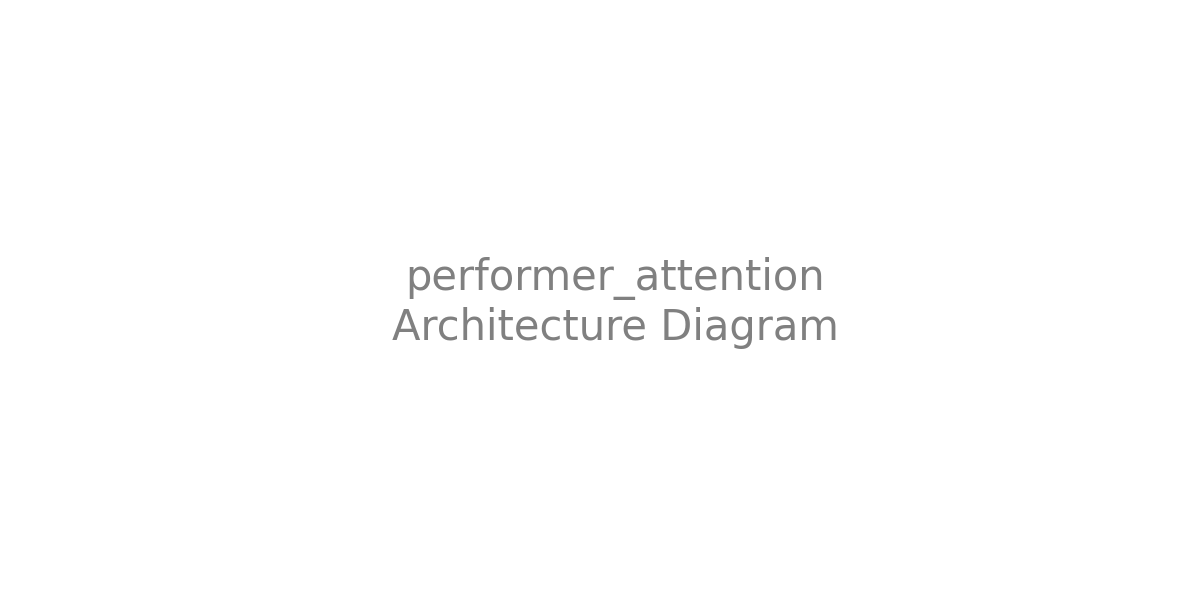
\includegraphics[width=\linewidth]{figures/architecture.png}
\caption{High-level architectural diagram of performer\_attention.}
\label{fig:arch\_performer-attention}
\end{figure}

